\section{Related Work}
\label{sec:related}
%To the best of our knowledge, there is no
The majority of existing research related to \textit{aspect-based review analysis} is about how to mine opinion based on given aspects~\cite{su2008hidden,zeng2013classification} or to jointly extract the aspects and sentiment~\cite{lin2009joint,qiu2011opinion,liu2016improving}. 
Their defined aspect extraction problem is to detect the aspect words in a given sentence, while ours is to extract the most prominent aspects from a large set of review sentences.
Some related work focuses on extracting aspect terms while most work does not aim to extract aspect terms or phrases for a particular product type.
Our work instead focus on extracting most prominent aspect terms from user reviews. 
We divide the existing work on this task into two types:
\begin{itemize}
	\item \textit{rule-based} methods, most of which utilize handcrafted rules to extract candidate aspects
	and then perform clustering algorithm on them.
	\item \textit{topic modeling based} methods, which directly model topics from texts and then extract aspects from 
	the topics.
\end{itemize}
\begin{figure*}[h!]
	\centering 
	{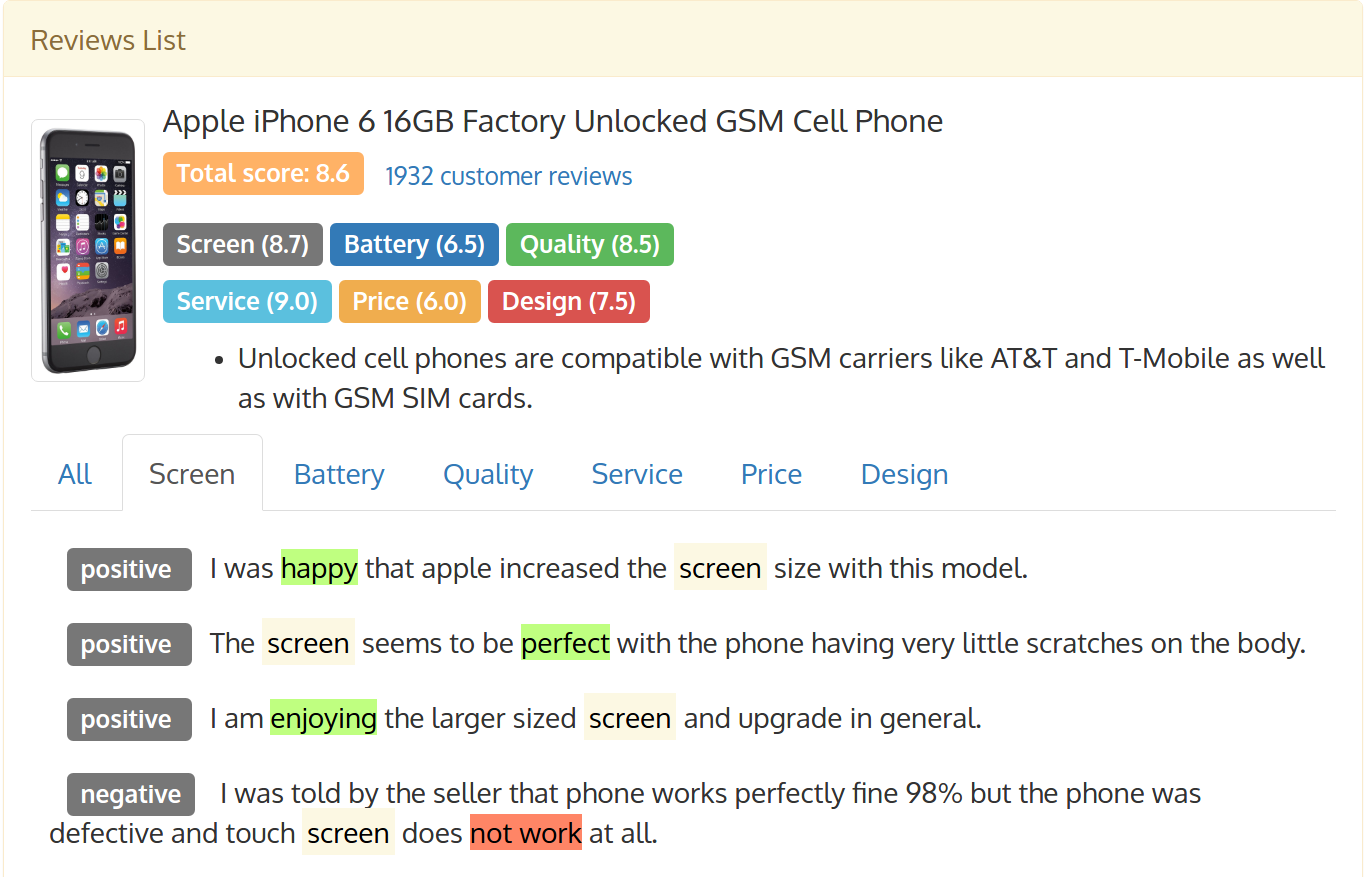
\includegraphics[width=1.5\columnwidth]{figures/sentimentexample.png}}
	\caption{Review snippets displayed by the aspects\label{fig:experiments:sentimentexample}}
\end{figure*}
%There is much existing work on aspect extraction and they can be 
%roughly divided in two categories. The first kind is predominately rule-based
%methods that find the aspect candidates first and then cluster them. 
%The second kind are mostly topic model approaches, which cluster the 
%aspect candidates and other words together, then identify the aspects.
\subsubsection{Rule-based Methods}
For rule-based methods, researchers leverage word statistical and syntactic features 
to manually design rules, recognizing aspect candidates from texts.
%Rule-based methods rely heavily on parsing and the quality of parsing. 
%Based on the parsing result, they use features such as frequency and 
%modifying relationship or a set of manually defined rules to identify 
%the aspect candidates.
% A problem with this kind of method is 
%\emph{implicit aspect extraction}, that is to find those aspect candidates 
%that are expressed without directly mentioning the aspect word. 
%For example in a mobile phone review ``Under heavy usage it will last 
%at least a day'' is about the aspect of battery life. Also co-reference 
%may be a problem as in this hotel review: ``I really liked the room. 
%It is large and comfy.'' 
%Rule-based methods need carefully designed rules 
%or other methods for implicit aspect extraction.
Some previous work proposed carefully designed rules 
for aspect extraction.
Poria et al. 2014 \cite{poria2014rule} uses manually crafted mining rules. 
Qiu et al. 2011 \cite{qiu2011opinion} also used rules, plus the 
Double Propagation method to better relate sentiment to aspects. 
Gindl et al. 2013 \cite{gindl2013rule} cooperate the Double Propagation 
 with anaphora resolution for identifying 
co-references to improve the accuracy. 
Su et al. 2008 \cite{su2008hidden} used a clustering method to map 
the implicit aspect candidates (which were assumed to be noun form 
of adjectives in the paper) to explicit aspects. 
Zeng et al. (2013)~\cite{zeng2013classification} mapped implicit features to explicit 
features using a set of sentiment words and by clustering explicit 
feature-sentiment pairs.
Rana et al. (2017)~\cite{rana2017two} propose a two-fold rules-based model, which uses rules defined on the basis of sequential patterns mined from customer reviews. Their first fold extracts aspects associated with domain independent opinions and the second fold extracts aspects associated with domain dependent opinions. 
However, the model is restricted by the pre-defined rules and thus does not scale well.
\subsubsection{Topic Modeling based Methods}
Topic models have been used to perform extraction and clustering 
at the same time. Most existing work are based on two basic models, 
pLSA\cite{hofmann1999probabilistic} and LDA\cite{blei2003latent}. 
Applying topic models on user reviews requires extra attention to
the nature of review texts. Two features of review texts are often considered 
in several modifications of topic model. The first feature is the 
quick shift of topics between sentences, since people express 
multiple opinions about various aspects within a short piece of text. 
Sentences close to each other may talk about completely different but 
related topics. Phrase-based LDA The other feature is the prominence of 
sentiment. Since reviews express opinions, naturally there are 
many sentiments, and also there is a strong relationship between the 
sentiments and the aspects. Many variations of LDA exploits this 
feature to improve the mining of aspects.
Lakkaraju et al. 2011 \cite{lakkaraju2011exploiting} models in 
parallel aspects and sentiments per review. 
Lin et al. 2009 \cite{lin2009joint} models the dependency between 
the latent aspects and ratings. Wang et al. 2011\cite{wang2011latent} proposed 
a generative model which incorporates topic modeling technique 
into the latent rating regression model\cite{wang2010latent}.
Moghaddam et al. 2012 \cite{moghaddam2012design} made a nice 
summarization of some basic variations of LDA for opinion mining.
Our method can be thought of as a hybrid approach with topic modeling as
one of its elements.
%\KZ{What exactly do the following approaches belong to: rule based or
%topic model, or in the middle. It's not very clear to me.}
%To improve the accuracy of the aspects or make use of cross-domain knowledge, several work introduced semi-supervised learning for aspect extraction. 
%\cite{mukherjee2012aspect} used a set of incomplete aspects as seeds and iteratively find more aspects. 
%\cite{andrzejewski2009incorporating} incorporate two forms of prior knowledge from the user: must-links and cannot-links. 
%\cite{chen2014aspect} automatically mined such information from cross-domain dataset.

He et al. (2017)~\cite{DBLP:conf/acl/HeLND17}  propose a neural attention model for identifying aspect terms, but their proposed model is unable to automatically extract the prominent ones from the \textit{representative terms}, which means they have to manually infer the main topics of the extracted terms.
Whereas, ExtRA extracts the most prominent aspect terms without human labor, namely the ``aspect labels'' in their paper.  
Also, their model does not support mining aspect phrases, while ExtRA can mine the valuable and informative phrases as target prominent aspects. 

%\KZ{It would be nice to give the ballpark of the rough accuracies of the above
%two approaches, so the audience knows where the baselines stand.} 
%Rule-based methods largely rely on parsing so the performance may vary according to the parser and the quality of dataset. Our method doesn’t need parsing for preprocessing and treat sentence as bag-of-word, so it won’t have that problem. Our method only uses the text from user reviews and is completely unsupervised, so we don’t require that the dataset contains information of ratings or that users provide seeds. 
%\KZ{Are we the first or the second kind. How are we
%different from the second (topic model) kind of approach? Not clear...}

%\ZY{Most recently, Wu et al. 2017 developed an aspect-based sentiment analysis system 
%
%}
Most previous work on aspect extraction utilizes variations of 
topic modeling, and aspects are modeled as topics, that is, 
word distributions. 
To the best of our knowledge, most previous work requires 
manual selection to choose the best word as a representative for 
each topic. 
For example in Titov et al. 2008 \cite{titov2008modeling}, 
the authors manually labeled each topic inferred from mp3 player reviews. 
On the contrary, our method is designed to automatically select the 
best words so that the whole process requires no human effort or labels. 
We argue that this is an important difference for real-world application, 
since selecting the best words for each product category is still 
too much effort for websites like Amazon and Yelp, while 
our method requires no manual processing and thus can be 
used directly for real-world applications like aspect-based 
review summarization. Moreover, such automatic aspect extraction enables
dynamic change of the aspect words over time to reflect changing customer
interest or taste.

Plus, the prominent aspect terms automatically extracted by our framework can be easily fed to downstream aspect-based review analysis and summarization frameworks. 
The aspect clusters generated by our model can be used for two purposes:
\begin{itemize}
    \item The top word of each cluster can be used as the basis of
          review summarization.
    \item The clusters can be used for identifying aspects in review texts.
\end{itemize}
In \secref{sec:demo} we used a simple neural network model to predict
the sentiment score for each aspect. More sophisticated  
neural network models for single sentence sentiment prediction
\cite{maas2011learning,socher2013recursive,dos2014deep,tang2015document}
can be used. 
They can form an automatic chain of software to
produce more accurate, quantitative review summaries from massive online reviews.
